\documentclass[a4paper]{article}

\usepackage[utf8]{inputenc}
\usepackage[T1]{fontenc}
\usepackage[italian]{babel}

\usepackage[margin=4.2cm, top=1.5cm, bottom=2.5cm]{geometry}

\usepackage{siunitx}
\usepackage{amsmath}
\usepackage{amssymb}
\usepackage{xfrac}
\usepackage{esint}
\usepackage[hidelinks]{hyperref}
\usepackage{graphicx}
\usepackage[font={sf}]{caption}
\usepackage{pdflscape}
\usepackage{makecell}
\usepackage{float}
\usepackage{subfig}
\usepackage{wasysym}
\usepackage{booktabs}

\setlength{\marginparwidth}{95pt}
\let\oldmarginpar\marginpar
\renewcommand\marginpar[1]{\oldmarginpar{\scriptsize\sffamily #1}}
\newcommand*\de{\mathrm{d}}
\newcommand*\pdv[2]{\frac{\partial #1}{\partial #2}}
\newcommand*\dv[2]{\frac{\de #1}{\de #2}}
\DeclareMathOperator\Ei{Ei}
\newcommand*\is{\equiv}
\newcommand\cs{$^{\text{137}}\text{Cs}$}
\newcommand\co{$^{\text{60}}\text{Co}$}
\newcommand\na{$^{\text{22}}\text{Na}$}
\newcommand\am{$^{\text{241}}\text{Am}$}
\newcommand\sr{$^{\text{90}}\text{Sr}$}

\sisetup{%
separate-uncertainty=true,
multi-part-units=single,
exponent-product=\cdot}

\frenchspacing

\title{Relazione di laboratorio:\\
Esperienza 4: Annichilazione del positrone}
\author{Andrea Marasciulli
\and Giacomo Petrillo
\and Roberto Ribatti}
\date{24 aprile -- 25 maggio 2018}

\begin{document}

\maketitle

\begin{abstract}

Misuriamo la massa dell'elettrone con una precisione maggiore dell'$1\permil$ facendo felice Punzi e (forse) il rate di cattura elettronica. Se siamo fortunati vediamo anche il positronio decadere in 3 fotoni.

\end{abstract}

{\tableofcontents}

\newpage
\section{Introduzione}

L'obiettivo principale dell'esperienza è la misura della massa del positrone sfruttando il decadimento $\beta^+$ del \na{}. Poi misuriamo l'efficienza dei rivelatori per stimare il rate di cattura elettronica rispetto al decadimento $\beta^+$. Infine cerchiamo di provare l'esistenza dell'annichilazione i 3 fotoni.

\section{Teoria}

\subsection{Spettro delle sorgenti a disposizione}

La nostra sorgente di \na{} ha 3 modi di decadimento:
\begin{itemize}
\item decadimento $\beta^+$ con $E_e=\SI{545}{keV}$, BR=90.4\%;
\item cattura elettronica (BR=9.5\% ) con la conseguente emissione di un fotone di energia \SI{1274}{keV} da parte del $^{22}$Ne formatosi;
\item decadimento $\beta^-$ con BR=0.1\%.
\end{itemize}

Useremo i decadimenti $\gamma$ del \cs{} (\SI{662}{keV}) e del \co{} (\SI{1173}{keV}, \SI{1332}{keV}) per calibrare il nostro apparato.

\marginpar{Scrivere perché non usiamo l'americio?}

\subsection{Fenomenologia dei rivelatori}

\marginpar{Scrivere materiale e dimensioni nella sezione ``apparato''}

Nel range di energie dei fotoni in cui lavoriamo, i processi di diffusione possibili sono gli scattering Rayleigh e Compton e l'effetto fotoelettrico.
Lo scattering Rayleigh, in quanto completamente elastico, non rilascia energia nel calorimetro.
Nella diffusione Compton il fotone cede una parte dell'energia ad un elettrone del nostro calorimetro e possiamo misurare l'energia persa da quest'ultimo. L'energia persa dal fotone segue la distribuzione di Klein-Nishina.
\marginpar{Klein-Nishina è la distribuzione angolare, non dell'energia.}
Se il fotone esegue un effetto fotoelettrico, perde tutta la sua energia cedendola ad un elettrone ed è l'unico modo che abbiamo per conoscere l'energia del fotone incidente.

A questo quadro si possono aggiungere processi di ordine superiore, come un numero maggiore di rimbalzi Compton all'interno del cristallo oppure un effetto fotoelettrico eseguito dopo uno scattering Compton.
Vedremo in seguito che un fotone, dopo aver eseguito un Compton all'interno di un rivelatore, può uscirne ed essere rivelato anche da un altro.

Riportiamo in \autoref{sezioni} un grafico che rappresenta la sezione d'urto dell'effetto Compton confrontata con quella del fotoelettrico all'interno del NaI. Per energie minori di \SI{300}{keV} l'effetto fotoelettrico domina sul Compton e viceversa per energie maggiori.
Trascuriamo la produzione di coppie perché, quando è sopra soglia ($E_{\gamma}>\SI{1}{MeV}$), è 5 volte più piccola della sezione d'urto del fotoelettrico che, in questo range, è molto soppressa rispetto al Compton.
\marginpar{La caption di \autoref{fig:cross} è poco chiara, $\lambda$ è quello del grafico ma non c'è scritto da nessuna parte.}

\begin{figure}[h]
\centering
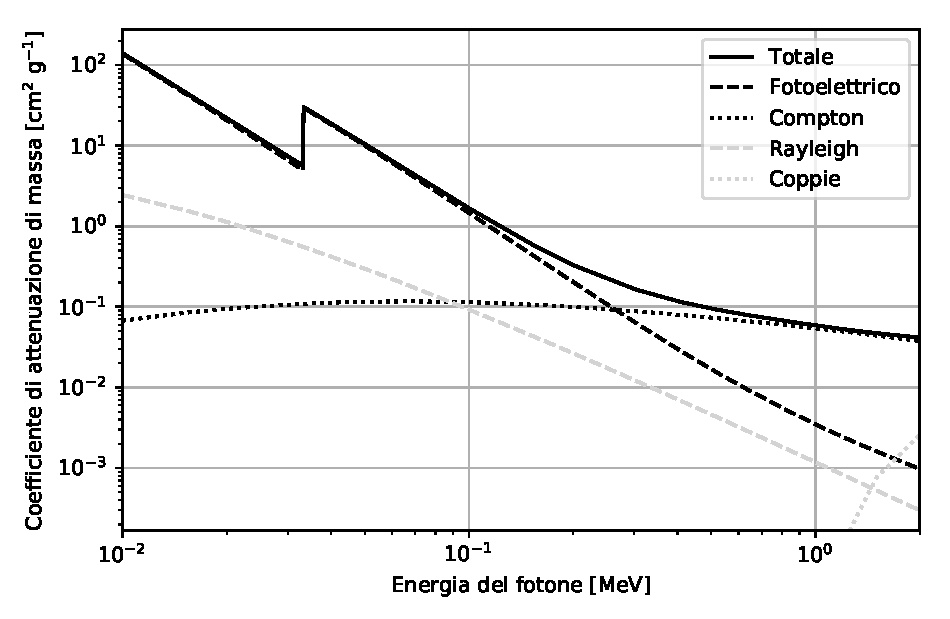
\includegraphics[width=25 em]{immagini/cross}
\caption{\label{fig:cross}
Sezioni d'urto in funzione dell'energia all'interno del nostro cristallo di NaI ($\rho=\SI{3.67}{g\,cm^{-3}})$ espressa come $\sigma=\frac{1}{\rho\lambda}$, dove $\lambda$ è il cammino libero medio all'interno del materiale. Queste informazioni sono tratte da \cite{cross}.}
\label{sezioni}
\end{figure}


\section{Misura e analisi}

\subsection{Stabilità}

Mostriamo l'instabilità del nostro sistema di rivelatori nei 2 apparati sopra descritti monitorando la posizione dei fotopicchi del sodio in funzione del tempo.
La prima misura è stata fatta con l'apparato A il 3 maggio e dura \SI{16}{ore}, la seconda  è stata eseguita con l'apparato B il 15 maggio e dura \SI{63}{ore}.
Nella prima misura sono presenti tutti i canali, nella seconda è presente solo il canale 1 per evitare il cross-talk riscontrato nella precedente.
Abbiamo usato l'energia nominale dei 2 picchi per ricavare una ``retta di calibrazione'' di pendenza $m$ e intercetta $q$ e abbiamo osservato l'evoluzione temporale di questi parametri. Usiamo l'espressione tra virgolette perché lo scopo dell'esperienza è fingere di non conoscere la massa dell'elettrone per poi misurarla.

% misura 1
\begin{figure}[h]
\centering
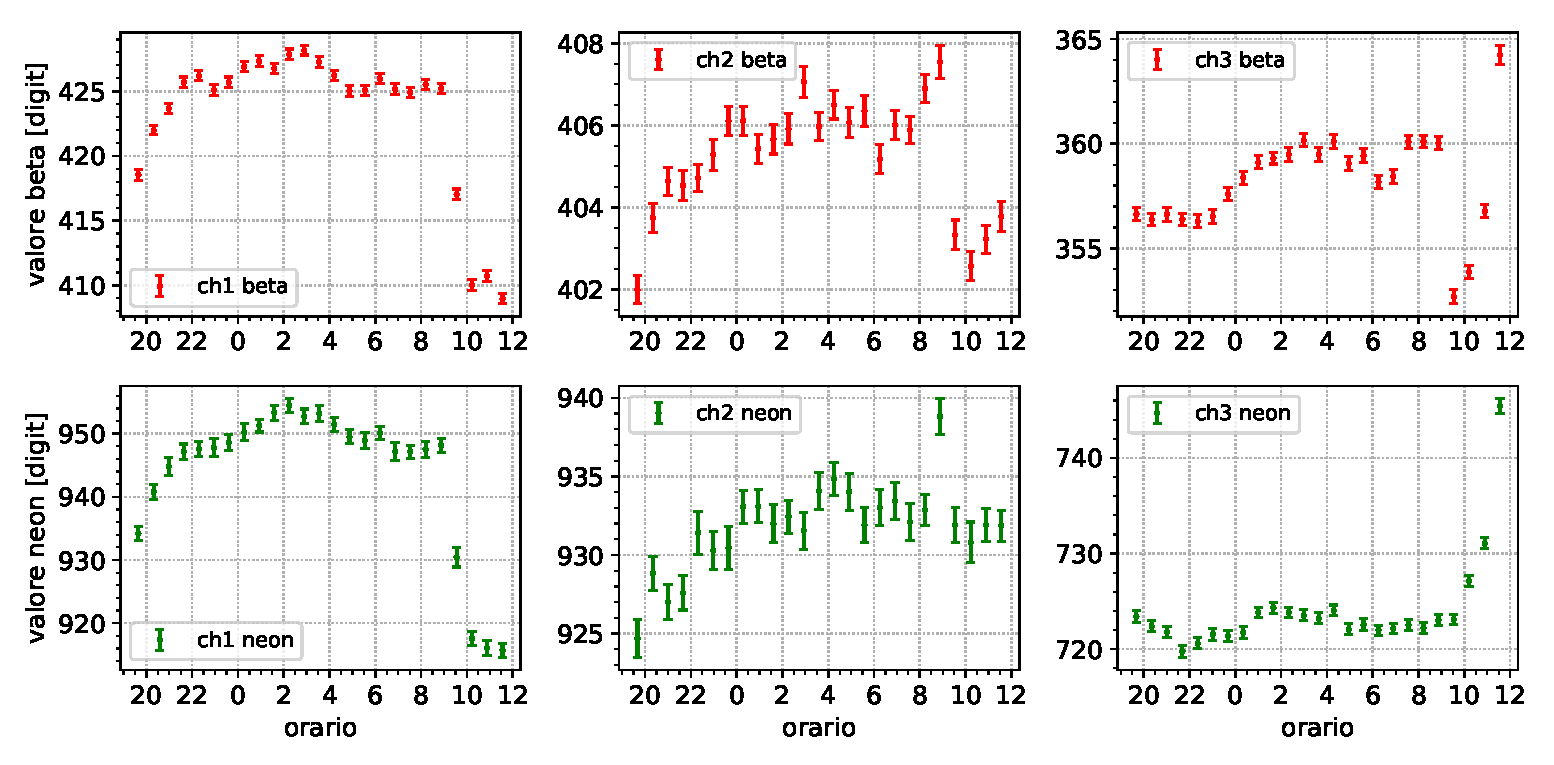
\includegraphics[width=\textwidth]{immagini/0503_picchi}
\caption{Misura di stabilità iniziata il 3 maggio alle 19. I grafici rappresentano la posizione dei picchi in funzione del tempo; ``beta'' indica il picco di annichilazione e ``neon'' indica il fotone emesso dal decadimento del neon.}
\label{picchi1}
\end{figure}

\begin{figure}[h]
\centering
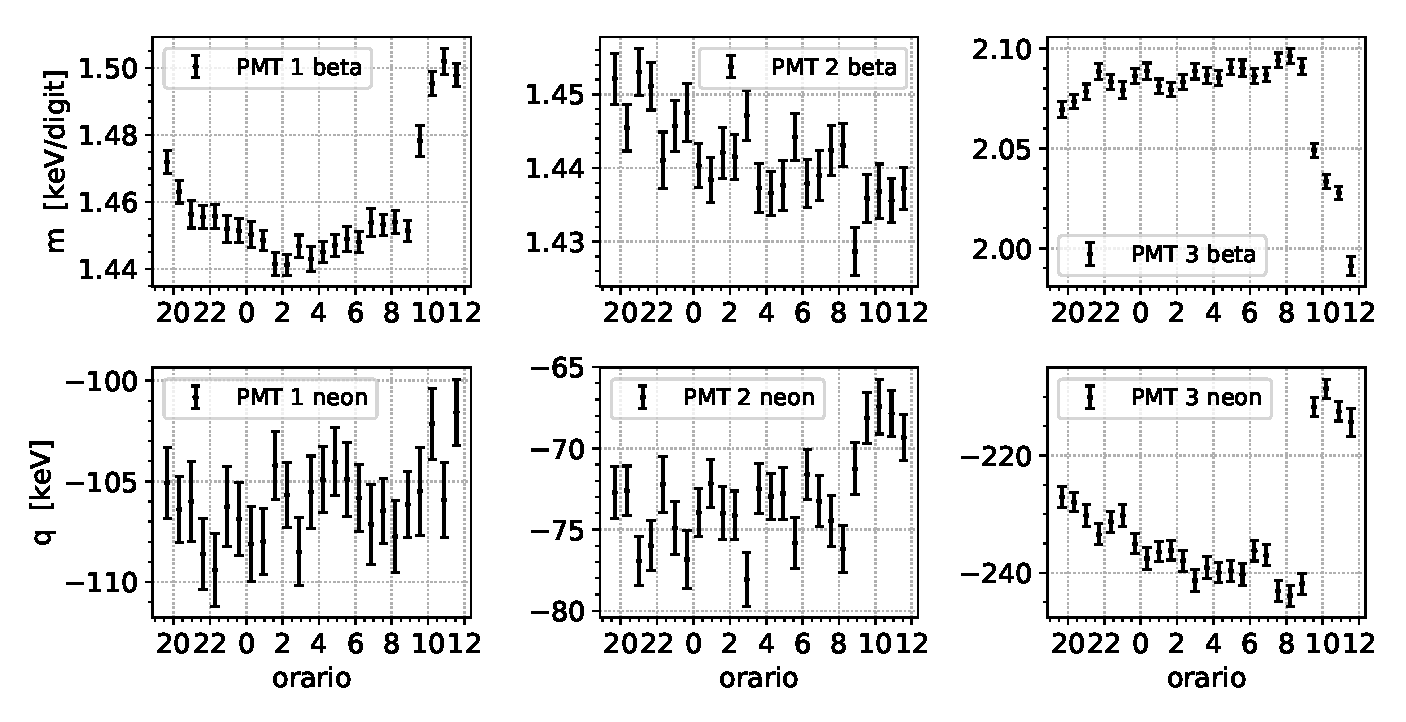
\includegraphics[width=\textwidth]{immagini/0503_rette}
\caption{Misura di stabilità iniziata il 3 maggio alle 19. I grafici rappresentano il valore della pendenza e dell'intercetta della ``retta di calibrazione'' in funzione del tempo.}
\label{rette1}
\end{figure}

% misura 2
\begin{figure}[h]
\centering
\subfloat
{
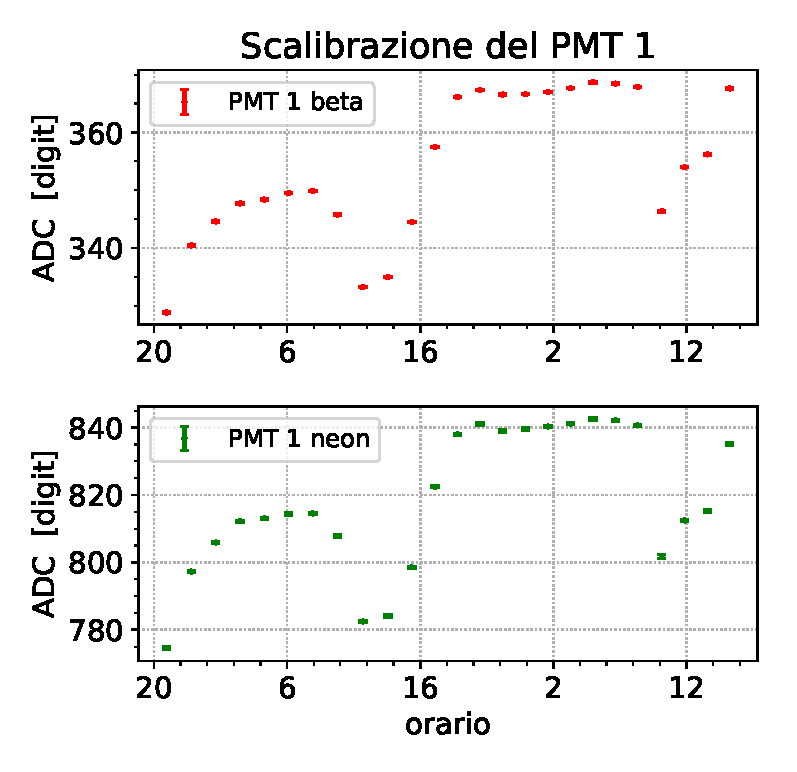
\includegraphics[width=0.49\textwidth]{immagini/0515_picchi}
}
\subfloat
{
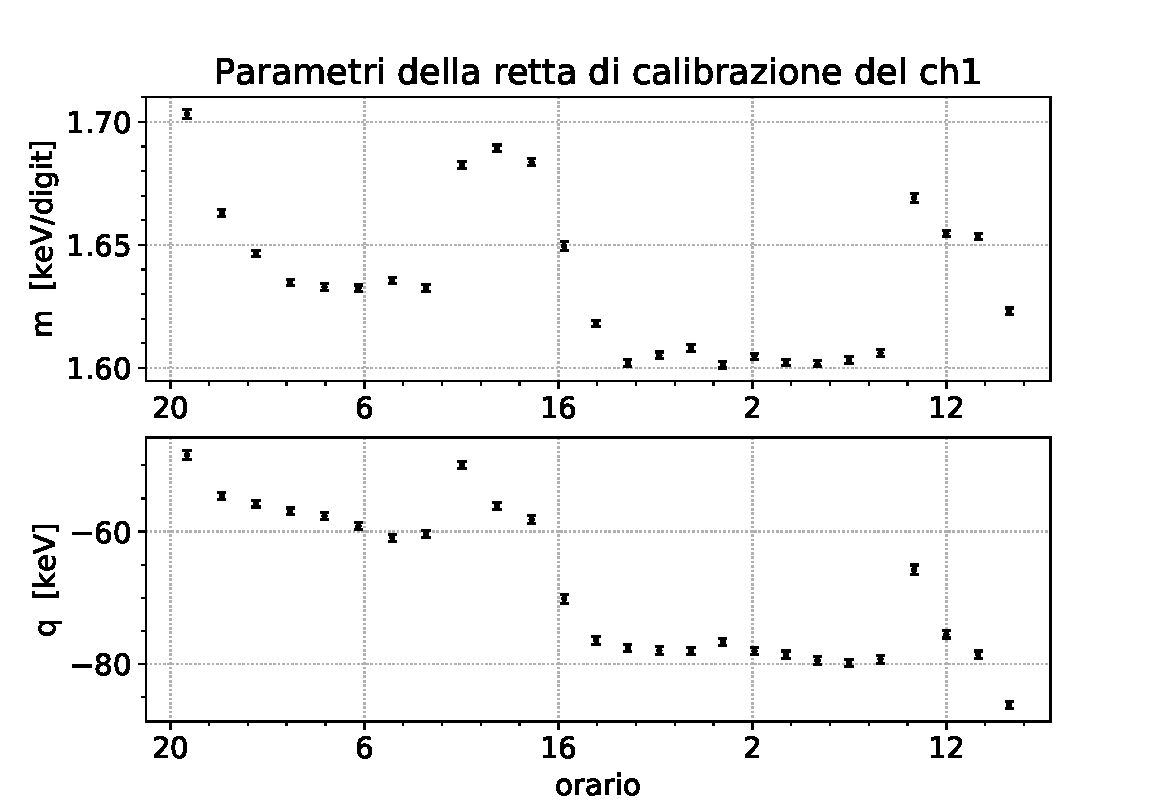
\includegraphics[width=0.49\textwidth]{immagini/0515_rette}
}
\caption{Misura di stabilità iniziata il 15 maggio alle 19.\\
A sinistra:  grafici che rappresentano la posizione dei picchi in funzione del tempo; ``beta'' indica il picco di annichilazione e ``neon'' indica il fotone emesso dal decadimento del neon. \\
A destra: grafici che rappresentano il valore della pendenza e dell'intercetta della ``retta di calibrazione'' in funzione del tempo.}
\label{picchi2}
\end{figure}

% discussione dei dati
Guardando i dati della prima misura (\autoref{picchi1} e \autoref{rette1}) vediamo che i vari rivelatori si scalibrano in modo diverso. L'andamento dei punti indica la notte come momento di massima stabilità e l'apertura del laboratorio come momento di massima instabilità.

Dai dati della seconda misura (\autoref{picchi2} sinistra e \autoref{picchi2} destra) si nota uno spostamento coerente dei fotopicchi del sodio che si stabilizza durante la notte. Anche qui si nota una scalibrazione significativa durante gli orari di apertura del laboratorio.
Le stesse considerazioni valgono anche per i parametri della retta di calibrazione.

\subsection{Misure con TDC}

Collegando le uscite discriminate dei PMT 1 e 2 ai due ingressi dell'unico TDC funzionante che abbiamo trovato in laboratorio, possiamo misurare i ritardi tra le risposte di due PMT posti uno di fronte all'altro sfruttando i fotoni dell'annichilazione. Per eseguire la misura usiamo come trigger le coincidenze e ritardiamo i segnali dei due PMT, dato che il trigger è successivo alla rivelazione dei fotoni. \`E stato scelto un ritardo di \SI{60}{ns} in modo che la differenza tra i tempi di arrivo $\Delta t=t_1-t_2$ possa essere sia positiva che negativa.

Prima di eseguire la misura calibriamo il TDC con il generatore di funzioni usando come trigger un'onda quadra e come \emph{stop} lo stesso segnale ma ritardato in modo arbitrario.
Eseguiamo questa calibrazione per le due scale disponibili: \SI{102}{ns} e \SI{510}{ns}.
Le calibrazioni hanno mostrato una buona linearità, ma la misura dei ritardi ha mostrato che il TDC, per un motivo a noi ignoto, non funziona.
Il grafico di Figura\autoref{100} è uguale a quello di Figura\autoref{500} nonostante le acquisizioni siano state fatte con due scale diverse. Se nei due grafici ci fosse la stessa cosa, vedremmo la figura allargata di un fattore dato dal rapporto dei due fondoscala. Inoltre l'offset delle scale del TDC vale circa \SI{1}{digit}, quindi lo spostamento di circa \SI{50}{digit} del picco presente nei grafici non può essere spiegato da nessun effetto fisico.

\begin{figure}[h]
\centering
\subfloat
{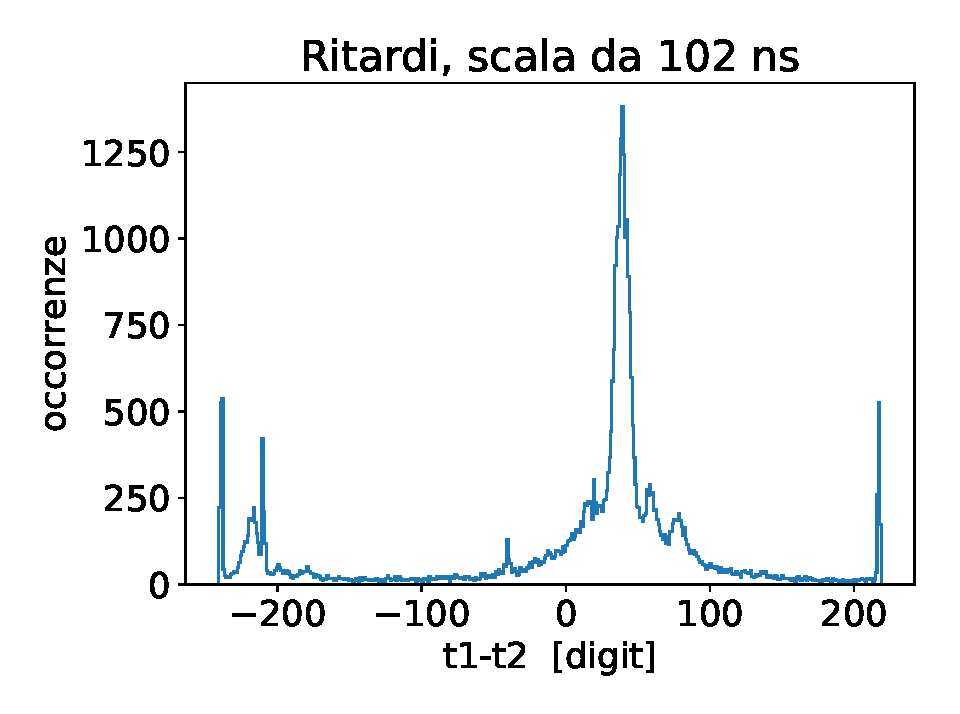
\includegraphics[width=17 em]{immagini/100}
\label{100}} \quad
\subfloat
{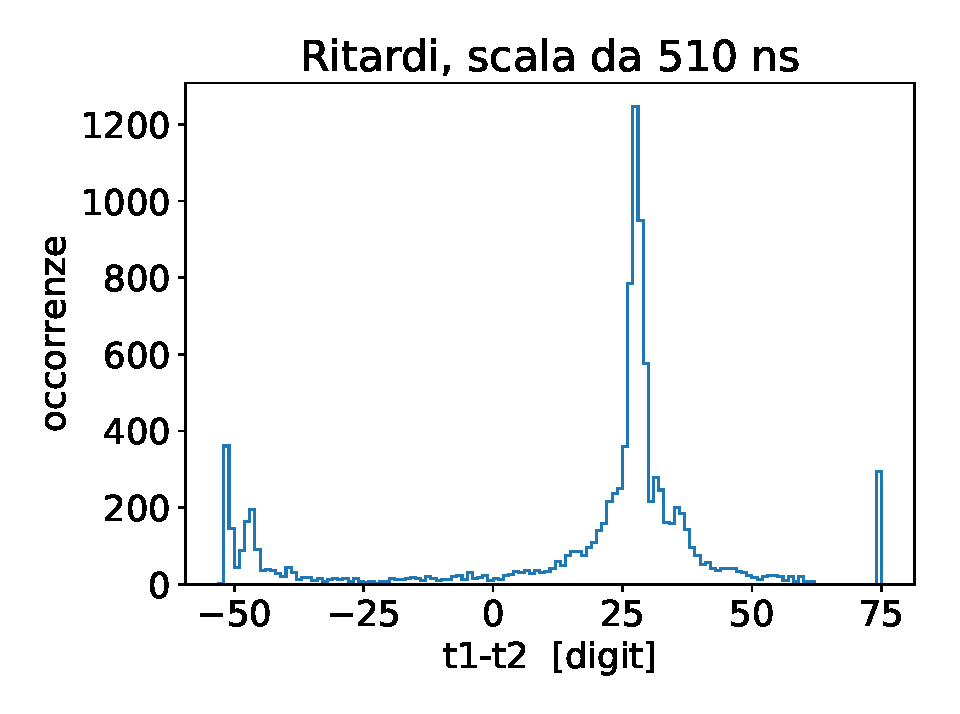
\includegraphics[width=17 em]{immagini/500}
\label{500}}

\caption{Misura di ritardo vista da entrambe le scale del TDC.}
\label{confronto}
\end{figure}

Questo problema ci impedisce di fare i facoltativi.

\begin{thebibliography}{99}

\bibitem[1]{cross}
M.J. Berger, J.H. Hubbell, S.M. Seltzer, J. Chang, J.S. Coursey, R. Sukumar, D.S. Zucker, and K. Olsen, XCOM: Photon Cross Sections Database, \emph{National Institute of Standards and Technology} (2010).

\end{thebibliography}

\appendix


\end{document}